\section{初值依赖}
\label{sec:odesens-initial}

定理~\ref{thm:odesens-basic-estimate}假设两条曲线都在$[t_0,T]$上存在，并且都留在同一个有Lipschitz常数的集合里。这对邻近初值的解并非自动成立。考虑$\dot{x}=x^2$，解是
\[
 x(t)=\frac{x_0}{1-x_0t},
\]
正初值的解在$t=1/x_0$爆炸。从$x_0=0.5$出发的解在$[0,1]$上存在，从$x_0=1.25$出发的解到$t=0.8$就没有了。

我们要回答的是：给定一条在紧区间$[t_0,T]$上存在的解，多近的初值能保证解也活到$T$，并且曲线距离可控？

\paragraph{在解的周围取一段管道}
思路是沿着已知解围一条半径为$\rho$的管道。管道是紧集，右端在里面有统一的Lipschitz常数。邻近的解只要还在管道里，Gronwall上界就成立；上界又说明它离中心线不超过$\rho/2$，碰不到管壁。图~\ref{fig:odesens-tube-continuation}中的红色虚线是一条假想的解，它要到达管壁，必须先穿过$\rho/2$的范围，这与上界矛盾。于是解出不去，也就活到了$T$。

\begin{BookInlineFigure}
  \centering
  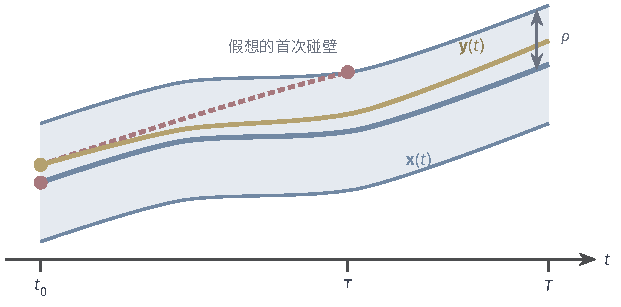
\includegraphics[width=105.2mm]{figures/06-differential-equations/01-ordinary-differential-equations/tikz/odesens-tube-continuation/figure.pdf}
  \caption{管道论证示意。浅蓝带是参考解$\bm{x}(t)$（蓝）周围半径$\rho$的管道，右端在其中有统一的Lipschitz常数。初值足够近的解$\bm{y}(t)$（黄）留在管道内。红色虚线表示假想的情形：解在$\tau$时首次碰壁，这与上界矛盾。}
  \label{fig:odesens-tube-continuation}
\end{BookInlineFigure}

图~\ref{fig:odesens-common-interval}的浅蓝带就是$\dot{x}=x^2$的管道。

\begin{BookInlineFigure}
  \centering
  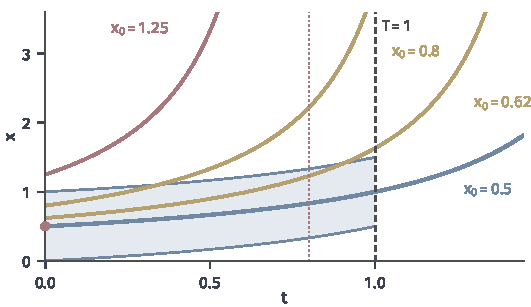
\includegraphics[width=90mm]{figures/06-differential-equations/01-ordinary-differential-equations/matplotlib/odesens-common-interval/figure.pdf}
  \caption{$\dot{x}=x^2$的邻近解。蓝色粗线从红点$x_0=0.5$出发，在$[0,1]$上存在，浅蓝带是半径$\rho=0.5$的管道。黄线$x_0=0.62$、$x_0=0.8$在$T=1$之前穿出管道，但解仍能活到$T=1$。红线$x_0=1.25$在红色点线$t=0.8$处爆炸，到不了$T=1$（灰色虚线）。}
  \label{fig:odesens-common-interval}
\end{BookInlineFigure}

证明要用第~\ref{chap:ode-existence-continuation}章的延拓结论：在局部唯一条件下，最大解若不能继续延拓，就会离开定义域内的任意紧集。也就是说，一段解如果始终留在定义域内的某个紧集里，就可以向后延伸。

\begin{theorem}[初值的局部Lipschitz依赖]
\label{thm:odesens-local-lipschitz}
设$\bm{D}\subseteq\mathbb{R}\times\mathbb{R}^{n}$是开集，$\bm{f}:\bm{D}\to\mathbb{R}^{n}$连续，且在每一点附近关于状态Lipschitz。设$\bm{x}:[t_0,T]\to\mathbb{R}^{n}$是一条解，其图像落在$\bm{D}$内。则存在$\rho>0$，使管道
\begin{equation}
 \bm{K}_\rho=\bigl\{(t,\bm{z}):t\in[t_0,T],\ \lVert\bm{z}-\bm{x}(t)\rVert_2\leq\rho\bigr\}
 \label{eq:odesens-tube}
\end{equation}
是$\bm{D}$的紧子集，$\bm{f}$在其上关于状态有统一的Lipschitz常数$L$。进一步，令$\delta=\tfrac12\rho\,\mathrm{e}^{-L(T-t_0)}$，则对每个满足$\lVert\bm{y}_0-\bm{x}_0\rVert_2\leq\delta$的$\bm{y}_0$，从$(t_0,\bm{y}_0)$出发的解在$[t_0,T]$上存在，且留在$\bm{K}_\rho$内。对两个这样的初值$\bm{y}_0$、$\bm{w}_0$，相应的解满足
\begin{equation}
 \lVert\bm{y}(t)-\bm{w}(t)\rVert_2\leq\mathrm{e}^{L(t-t_0)}\lVert\bm{y}_0-\bm{w}_0\rVert_2,\qquad t\in[t_0,T].
 \label{eq:odesens-local-lipschitz}
\end{equation}
\end{theorem}

\begin{proof}
先取管道。$\bm{x}$的图像是开集$\bm{D}$中的紧集，到$\bm{D}$的补集有正距离（$\bm{D}$是全空间时距离视为无穷）。取$\rho$小于这个距离的一半，则$\bm{K}_\rho\subset\bm{D}$，且$\bm{K}_\rho$是有界闭集，因而紧。

再说明Lipschitz常数统一。假设不然，对每个$k$有$(t_k,\bm{a}_k),(t_k,\bm{b}_k)\in\bm{K}_\rho$，使
\[
 \lVert\bm{f}(t_k,\bm{a}_k)-\bm{f}(t_k,\bm{b}_k)\rVert_2>k\lVert\bm{a}_k-\bm{b}_k\rVert_2.
\]
连续函数$\bm{f}$在紧集上有界，设界为$M$，于是$\lVert\bm{a}_k-\bm{b}_k\rVert_2<2M/k\to0$。取子列使两组点收敛到同一点$(t_\ast,\bm{z}_\ast)\in\bm{K}_\rho$。该点附近$\bm{f}$关于状态有Lipschitz常数，而$k\to\infty$与之矛盾。

现在设$\lVert\bm{y}_0-\bm{x}_0\rVert_2\leq\delta$，$\bm{y}$是最大解。令$\tau$为使$\bm{y}$在$[t_0,s]$上存在并留在$\bm{K}_\rho$内的$s\leq T$的上确界，初值在管道内部，所以$\tau>t_0$。在$[t_0,\tau)$上用定理~\ref{thm:odesens-basic-estimate}，$\bm{r}=\bm{0}$，得到
\[
 \lVert\bm{y}(t)-\bm{x}(t)\rVert_2\leq\mathrm{e}^{L(t-t_0)}\delta\leq\frac{\rho}{2}.
\]

这段解留在紧集$\bm{K}_\rho$内，由延拓结论，它可以延拓到$\tau$，且若$\tau<T$还能继续延拓到$\tau$之后。上面的不等式到$\tau$处仍成立，$\bm{y}(\tau)$离中心线不超过$\rho/2$，延拓后的一小段仍在管道内，与$\tau$的定义矛盾。所以$\tau=T$，解在闭区间$[t_0,T]$上存在且在管道内。

最后，两条解$\bm{y}$、$\bm{w}$都在$\bm{K}_\rho$内，再用一次定理~\ref{thm:odesens-basic-estimate}，就得到式~\eqref{eq:odesens-local-lipschitz}。
\end{proof}

定理中的量词值得留意。$\rho$、$L$、$\delta$都依赖给定的解和$T$，结论只在这条解附近成立，即使$\bm{f}$全局光滑也是如此。$T$越靠近这条解的爆炸时刻，管道内的$L$越大，$\delta$越小。

\begin{example}[管道的具体数字]
\label{ex:odesens-tube}
对$\dot{x}=x^2$，$x_0=1/2$，$T=1$，解$x(t)=1/(2-t)$取值在$[1/2,1]$内。取$\rho=1/2$，管道内状态在$[0,3/2]$中，$\lvert\partial_xf\rvert=2\lvert x\rvert\leq3$，所以取$L=3$。定理给出
\[
 \delta=\frac12\cdot\frac12\,\mathrm{e}^{-3}\approx0.0124.
\]

取$y_0=0.51$，它满足条件。上界给出
\[
 \lvert y(1)-x(1)\rvert\leq0.01\,\mathrm{e}^{3}\approx0.201.
\]
真实值可以直接算，
\[
 y(1)-x(1)=\frac{0.51}{0.49}-1\approx0.0408.
\]
上界偏大约五倍，因为它用整条管道上最坏的$L$。$\delta$也偏保守：实际上任何$y_0<1$的解都能活到$T=1$。定理的作用是不解方程也给出保证。
\end{example}

\paragraph{连续依赖与Lipschitz依赖}
定理~\ref{thm:odesens-local-lipschitz}的结论是\term{Lipschitz依赖}（Lipschitz dependence）：解的差不超过初值差的常数倍。更弱的要求是\term{连续依赖}（continuous dependence）：对任意$\varepsilon>0$，存在$\delta>0$，初值差小于$\delta$时，$[t_0,T]$上的解差小于$\varepsilon$。两者在依赖的“速度”上不同，所需条件也不同，见表~\ref{tab:odesens-dependence}。

\begin{BookInlineTable}
  \centering
  \caption{初值依赖的层次。结论都是给定解附近、紧时间段上的局部结论。}
  \label{tab:odesens-dependence}
  \begin{tabular}{p{28mm}p{32mm}p{38mm}}
    \toprule
    右端条件 & 依赖性质 & 例子 \\
    \midrule
    连续，解不唯一 & 流映射没有定义 & $\dot{x}=2\sqrt{\lvert x\rvert}$ \\
    连续，解唯一 & 连续依赖 & $\dot{x}=-x\ln\lvert x\rvert$ \\
    局部Lipschitz & Lipschitz依赖 & $\dot{x}=\lvert x\rvert$ \\
    连续可微 & 可微依赖（第~\ref{sec:odesens-variational}节） & $\dot{x}=x(1-x)$ \\
    \bottomrule
  \end{tabular}
\end{BookInlineTable}

第二行的结论是：右端仅连续时，只要过每个邻近初值的解都唯一，连续依赖仍然成立。证明需要用到等度连续曲线族的紧性（Arzelà--Ascoli定理）并配合延拓，篇幅较长，读者可查阅常微分方程教材。其机制是：邻近初值的解构成一族等度连续的曲线，任何收敛子列的极限都是初值问题的解，唯一性迫使极限只能是原来那条解。这个论证没有给出收敛的速度。

没有速度保证的情形确实存在。方程$\dot{x}=-x\ln\lvert x\rvert$（约定在$x=0$处右端为$0$）在$x=0$处斜率趋于无穷，右端不Lipschitz，但解仍唯一。对$0<x_0<1$，令$v=\ln x$，方程化为$\dot{v}=-v$，于是
\[
 x(t)=x_0^{\mathrm{e}^{-t}}.
\]
若有解从$0$离开，变量$v$要在有限时间内从$-\infty$变为有限值，而$\dot{v}=-v$的解不会在有限时间内从无穷回来，所以$x\equiv0$是从$0$出发的唯一解。

取$t=\ln2$，解的映射是$x_0\mapsto\sqrt{x_0}$。$x_0=10^{-4}$时解是$10^{-2}$，初值差被放大$100$倍；$x_0=10^{-8}$时放大$10^{4}$倍。比值$\sqrt{x_0}/x_0$没有上界，所以不存在Lipschitz常数。依赖仍然连续，因为$x_0\to0$时$\sqrt{x_0}\to0$，见图~\ref{fig:odesens-holder-flow}。

\begin{BookInlineFigure}
  \centering
  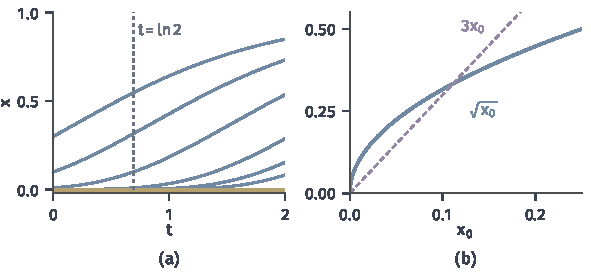
\includegraphics[width=100mm]{figures/06-differential-equations/01-ordinary-differential-equations/matplotlib/odesens-holder-flow/figure.pdf}
  \caption{连续依赖但不Lipschitz。(a)$\dot{x}=-x\ln x$从$x_0=10^{-8},10^{-6},10^{-4},10^{-2},0.1,0.3$出发的解（蓝）和零解（黄）。极小的初值很快被拉开。(b)$t=\ln2$时的解映射$\sqrt{x_0}$，在$x_0=0$处切线竖直，任何直线（紫色虚线）在原点附近都压不住它。}
  \label{fig:odesens-holder-flow}
\end{BookInlineFigure}

\paragraph{有限时间上界不是长期稳定判据}
式~\eqref{eq:odesens-local-lipschitz}的常数$\mathrm{e}^{L(T-t_0)}$随$T$指数增长。它只是有限时间的上界，不能用来判断解在长时间下靠拢还是分离。图~\ref{fig:odesens-bound-vs-true}用$L=1$的三个方程作对比，初值差都是$0.01$。

\begin{BookInlineFigure}
  \centering
  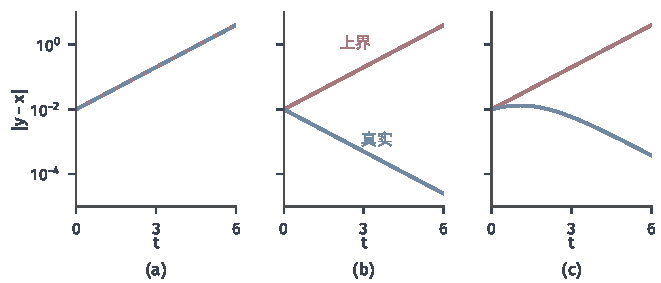
\includegraphics[width=112mm]{figures/06-differential-equations/01-ordinary-differential-equations/matplotlib/odesens-bound-vs-true/figure.pdf}
  \caption{同一个上界$0.01\,\mathrm{e}^{t}$（红）与三种真实距离（蓝，对数纵轴）。(a)$\dot{x}=x$，上界就是真实距离。(b)$\dot{x}=-x$，真实距离按$\mathrm{e}^{-t}$衰减。(c)$\dot{x}=x(1-x)$，$x_0=0.25$，距离先增后减。}
  \label{fig:odesens-bound-vs-true}
\end{BookInlineFigure}

三种情形的$L$相同，长期行为却完全不同，因为$L$只记录了$\lvert\partial_xf\rvert$的大小，丢掉了符号。反过来，$\mathrm{e}^{L(T-t_0)}$在任何固定的$T$上都有限，这也不说明解在$T\to\infty$时保持靠近。长期行为需要吸引性、不变集等额外结构，可参考\BookChapterRef{chap:dynamical-systems-long-term}{卷九第1章“动力系统与轨迹的长期行为”}。

\paragraph{保留符号信息}
能否在估计里留下符号？引理~\ref{lem:odesens-gronwall}的积分形式要求$\beta\geq0$，但如果直接对距离的平方求导，放大率可以取负。为此把Lipschitz条件换成只约束相互靠近方向的条件，称为\term{单侧Lipschitz条件}（one-sided Lipschitz condition）。

\begin{lemma}[单侧Lipschitz估计]
\label{lem:odesens-one-sided}
设$\bm{x},\bm{y}:[t_0,T]\to\bm{K}$绝对连续，几乎处处满足$\dot{\bm{x}}=\bm{f}(t,\bm{x})$、$\dot{\bm{y}}=\bm{f}(t,\bm{y})$。设实值函数$\mu$可积（可以取负值），且对几乎每个$t$及所有$\bm{a},\bm{b}\in\bm{K}$，
\begin{equation}
 \bigl\langle\bm{f}(t,\bm{a})-\bm{f}(t,\bm{b}),\,\bm{a}-\bm{b}\bigr\rangle\leq\mu(t)\lVert\bm{a}-\bm{b}\rVert_2^2.
 \label{eq:odesens-one-sided}
\end{equation}
则对每个$t\in[t_0,T]$，
\begin{equation}
 \lVert\bm{y}(t)-\bm{x}(t)\rVert_2\leq\lVert\bm{y}_0-\bm{x}_0\rVert_2\,\exp\int_{t_0}^{t}\mu(s)\,\mathrm{d}s.
 \label{eq:odesens-one-sided-bound}
\end{equation}
\end{lemma}

\begin{proof}
令$v=\lVert\bm{y}-\bm{x}\rVert_2^2$，$v$绝对连续。由式~\eqref{eq:odesens-one-sided}，几乎处处有
\[
 \dot{v}=2\bigl\langle\bm{f}(t,\bm{y})-\bm{f}(t,\bm{x}),\,\bm{y}-\bm{x}\bigr\rangle\leq2\mu v.
\]
记$M(t)=\int_{t_0}^{t}\mu$，乘以积分因子后得到
\[
 \frac{\mathrm{d}}{\mathrm{d}t}\bigl(\mathrm{e}^{-2M}v\bigr)\leq0.
\]
所以$v(t)\leq\mathrm{e}^{2M(t)}v(t_0)$，开方即得结论。
\end{proof}

对$\dot{x}=-x$，条件式成立且$\mu=-1$，式~\eqref{eq:odesens-one-sided-bound}恰好是真实的$\mathrm{e}^{-t}$衰减。对$\dot{x}=-x^3$，
\[
 (a-b)(-a^3+b^3)=-(a-b)^2(a^2+ab+b^2)\leq0,
\]
可取$\mu=0$，而这个右端在$\mathbb{R}$上没有全局Lipschitz常数。这样的方程上任意两条解的距离不增，这比用$L$的上界强得多。该结论同样只陈述了给定时间段上的比较，并不涉及平衡点的吸引。
